\bartchapterimage{heic0506a.jpg}
\chapter{SDSS-DR10 analysis}
\label{cha:sdss}
\bartthumb{heic0506a.png}
\minitoc%

\section{Introduction}

An application of MAGGIE on a real galaxy survey implies an analysis of the
galaxy sample. We must understand the various incompletenesses it suffers in
order to be able to correct them. Here we describe the analysis we performed on
the Sloan Digital Sky Survey, with the various problems we encountered.

\section{Analysis}

\subsection{Definitions}

In SDSS, strips are bands of observations along great circles of the survey.
Each of them is composed of six parallel scanlines (of 13 arcmin wide) with
gaps of approximately the same width between them. Two strips make a single
stripe of 2.5°. Each scanline include all the data (in $ugriz$), and is divided
in fields (that can overlap). So when accessing an observation at a given
position in the sky, we access a specific field. A given observation is
completely defined by its run number, the number of the camcol of the scanline
and by the field number.

The pipeline of the SDSS is applied for the objects extraction. They are
detected as pixel over-densities relative to the background. With this method,
multiple real and different objects can be seen as a single object. They are
linked by their pixels as galaxies using Friends-of-Friends algorithm. A
deblending algorithm is then applied to resolve child objects from their
parents (defined as the first detection). Then a resolve algorithm is applied
to extract the best object when multiple fields are overlapping.

There are numerous object flags that are useful to select well observed
galaxies. In the \texttt{PhotoObjAll} table, there is a \texttt{clean} for a
predefined selection of the most common good flags, which facilitates the
selection of galaxies.

There can be many problems with the photometry, with cases of bright galaxies
with sky levels not well estimated and missing faint galaxies for example. Most
of these known problems are corrected in the recent releases (DR9 and DR10).

Old releases worked with a spectrograph of 640 fibers, with collisions at
$55''$, while the new BOSS survey works with a 1000-fiber spectrograph but with a
greater collision size of $64''$. The coverage of the old releases should be
used for the new BOSS, so its better to use latest releases. Moreover, the
pipeline used for the spectrum had changed and improved along releases.

Following definitions given in the SDSS website, we can define two
coordinate systems in the survey.
%
\begin{description}
    \item[Great Circle:] This coordinates system is define with two angles
        $(\mu, \nu)$. Coordinates are relatives to one stripe so they can be
        used when working with galaxies inside a stripe region.

    \item[Survey Coordinates:] It's an other system similar to celestial
        coordinates but ``centred'' on the contiguous block of galaxies  of
        the survey. Coordinates are written $(\lambda, \eta)$. The range of
        these coordinates is: $-\cfrac{\pi}{2}<\eta<\cfrac{\pi}{2}$ and
        $-\pi<\lambda<\pi$.
\end{description}
%
We will work only with survey coordinates as they allow us to easily define
a mask for the SDSS\@. The celestial coordinates and survey coordinates are
the same system of coordinates, except that one is a particular rotation of
the other. The relations between the two systems are:

\subsubsection{Survey coordinates to celestial coordinates}

\begin{eqnarray}
    \delta &=&
        \arcsin\left(\cos\lambda\sin\left(\eta+\delta_0\right)\right)
        \nonumber\\
    \alpha &=&
        \mathrm{atan2}
        \left(\sin\lambda,\cos\lambda\cos\left(\eta+\delta_0\right)\right)+
        \alpha_0\nonumber\\
\end{eqnarray}
%
with ${\left(\alpha_0,\delta_0\right)}_{\left(\alpha,\delta\right)}=
{\left(185°,32.5°\right)}_{\left(\alpha,\delta\right)}=
{\left(0,0\right)}_{\left(\lambda, \eta\right)}$.

\subsubsection{Celestial coordinates to survey coordinates}

The inverse transformation is:
%
\begin{eqnarray} \eta &=& \mathrm{atan2}
\left(\sin\delta,\cos\delta\cos\left(\alpha-\alpha_0\right)\right)-
\delta_0\nonumber\\ \lambda &=&
\arcsin\left(\cos\delta\sin\left(\alpha-\alpha_0\right)\right) \nonumber\\
\end{eqnarray}
%
with ${\left(\alpha_0,\delta_0\right)}_{\left(\alpha,\delta\right)}=
{\left(185°,32.5°\right)}_{\left(\alpha,\delta\right)}=
{\left(0,0\right)}_{\left(\lambda,\eta\right)}$. Periodic conditions must be
applied to angles found by the latter equation:
%
\begin{equation} \begin{cases} \eta\rightarrow\eta+180° \;
    \lambda\rightarrow180°-\lambda& \mbox{if}\;\eta<-90°\;\mbox{or}\;
    \eta>90°\\ \eta\rightarrow\eta-360° & \mbox{if}\;\eta>180°\\
    \lambda\rightarrow\lambda-360° & \mbox{if}\;\lambda>180°\\ \end{cases}
\end{equation}
%
\subsubsection{Stripe number}
%
Stripes have a constant width of 2.5° along the $\eta$ coordinate. So, stripe
number $n$ of a galaxy with $\eta$ coordinate is:
%
\begin{equation} n = \mathrm{floor}\left(\cfrac{\eta+58.75°}{2.5°}\right)
\end{equation}
%
\subsection{Galaxy selection}
%
Many tables in the SDSS save galaxies and other objects properties extracted
from images of the survey. These tables are the results of different selections
in objects extracted in images. When crossing objects between images of the
survey that overlap, there are some differences in positions for the same
object. So there are possibilities that an object is observed twice or more. In
many of those tables, there is no object duplicated.

In the SDSS database, the \texttt{Galaxy} view is a selection from the
\texttt{PhotoPrimary} for objects flagged as \emph{galaxy}, with
\texttt{type}=3. The \texttt{Galaxy} view contains the photometric parameters
(no redshifts or spectroscopic parameters) measured for resolved primary
objects. But we have other useful informations to link with tables that give us
photometric and spectroscopic redshifts. There is the \texttt{specobjid} entry
to link with spectroscopic redshifts in the table \texttt{SpecObj} which
doesn't contain duplicates (it's a clean table of \texttt{SpecObjAll} with
clean redshifts). If \texttt{specobjid=0}, the galaxy doesn't have a
spectroscopic redshift (the galaxy wasn't spectroscoped). The \texttt{objid}
allows to link to the \texttt{Photoz} table which contains all photometric
redshifts for galaxies in the \texttt{Galaxy} table. Estimation is based on a
robust fit on spectroscopically observed objects with similar colors and
inclination angle. There is also the \texttt{PhotozRF} where estimates are
based on the Random Forest technique. Galaxies in the SDSS are limited to
$m_r<17.77$ and a given surface brightness. So we need to apply the same flux
limitations when selecting galaxies on the \texttt{Galaxy} table. A possible
\texttt{SQL} query for selecting galaxies in this table and link them with
redshift tables is for spectroscoped galaxies:
%
\begin{listing}[H]
    \begin{minted}[bgcolor=griscode, linenos]{sql}
SELECT G.ra, G.dec, G.petroMag_u, G.petroMag_g, G.petroMag_r,
G.petroMag_i, G.petroMag_z, G.specobjid, G.objid, Z.z, Z.Zerr
FROM Galaxy AS G
JOIN SpecObj AS Z ON Z.specobjid=G.specobjid
WHERE G.specobjid!=0
AND G.petroMag_r-G.extinction_r<17.77
    \end{minted}
\end{listing}
%
and for galaxies which couldn't be spectroscoped:
%
\begin{listing}[H]
    \begin{minted}[bgcolor=griscode, linenos]{sql}
SELECT G.ra, G.dec, G.petroMag_u, G.petroMag_g, G.petroMag_r,
G.petroMag_i, G.petroMag_z, G.specobjid, G.objid, Z.z, Z.Zerr
FROM Galaxy AS G, Photoz AS Z
WHERE G.specobjid=0
AND G.objid=Z.objid
AND G.petroMag_r-G.extinction_r<17.77
    \end{minted}
\end{listing}

Stripe limits are given in the table \texttt{StripeDefs} but they represents
the limits that were planned at the beginning of the survey, not the actually
observed limits.

Some planned regions aren't still observed, so we need to define other limits
in $\lambda$ coordinates for incomplete stripes. We find, by hand, the new
limits of stripes which contains spectroscoped galaxies. Now, the survey mask
is like in \bartreffigure{sdss}. We will consider just galaxies in this mask in
order to find groups in the SDSS\@.
%
\begin{figure}[ht] \centering
    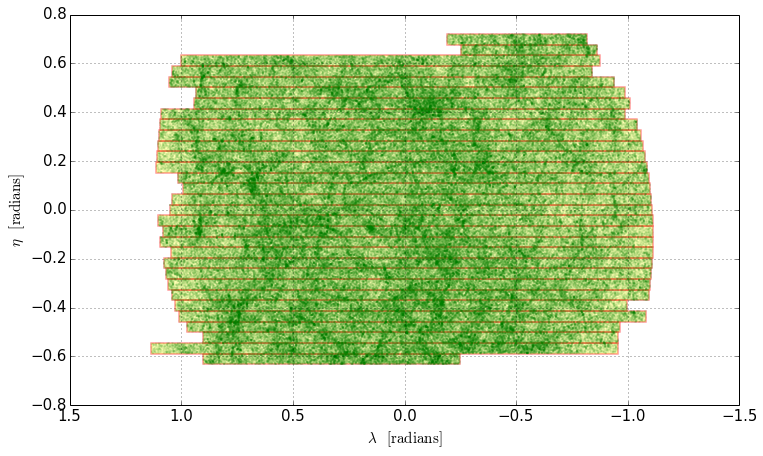
\includegraphics[width=\linewidth]{figures/sdss/sdss.png}
    \caption{Galaxies in the SDSS DR10 with stripes limits defined by hand. The
    red lines limits of the stripes make the SDSS mask used to identify
edges.\label{fig:sdss}}
\end{figure}

\subsubsection{Flags in the SDSS}

Galaxy photometry can have some troubles in the SDSS\@. In the general case,
those objects are flagged with \texttt{clean} property which indicates by 1
that the photometry is OK and by 0 when there is a problem. Details of the
problems are in the bit flag. But for groups, we need to select all galaxies,
even if they are not clean, or our groups will suffer incompleteness in their
membership and their physical properties such as luminosity, stellar mass\ldots
will be biased.

However, we have to take into account the error on the redshift estimation
using \texttt{zErr}. For photometric redshifts, if \texttt{zErr} is too high,
we can use \texttt{nnAvgZ}, which is the average redshift of galaxies in the
neighbourhood of the considered galaxy. It can be better if the photometric
redshift is strongly different from its value.

\texttt{SpecObjAll} contains duplicates and bad data. But \texttt{SpecObj}
contains just clean spectra. The field \texttt{zWarning} can be used to decide
if we keep a redshift or not.

\subsection{Fibre collision estimation}

We need a sample of galaxies for which we can easily characterize borders and
where all galaxies are present given the flux limit of the survey. But there is
the problem of missing galaxies due to fibre collisions. But our algorithm is
tested on a ``perfect'' mock catalogue. In order to know the behaviour of the
algorithm with these problematic galaxies, we need to implement the effect of
fibre collisions in our mock catalogue.

In the SDSS, galaxy spectra are obtained on fibers using a plate of 1.5°
diameter. But on the plate, the number of fibres is limited. Moreover, each
portion of the sky can't be respectroscoped multiple times, because the SDSS
had to cover a predefined portion of the sky in a fixed number of years.
Although spectroscopic runs may overlap, there are galaxies that can't be
spectroscoped. Indeed, while fibres collect spectra in a $3''$ diameter field,
their coatings prevent two fibres of lying close than $55''$ from one another.
When galaxies are closer than this distance, one (or more) of those galaxies
aren't spectroscoped. We can see this fibre collision effect in
\bartreffigure{plane}, where we have taken the nearest neighbour of a galaxy on
the celestial sphere, and determined the differences in angular positions and
redshift between the two galaxies. As expected, the number of galaxies that are
closer than $55''$ is much less than what would be extrapolated from greater
separations. There are still some galaxies because the overlapping of runs
allows to observe galaxy spectra below this limit.

\begin{figure}[ht] \centering
    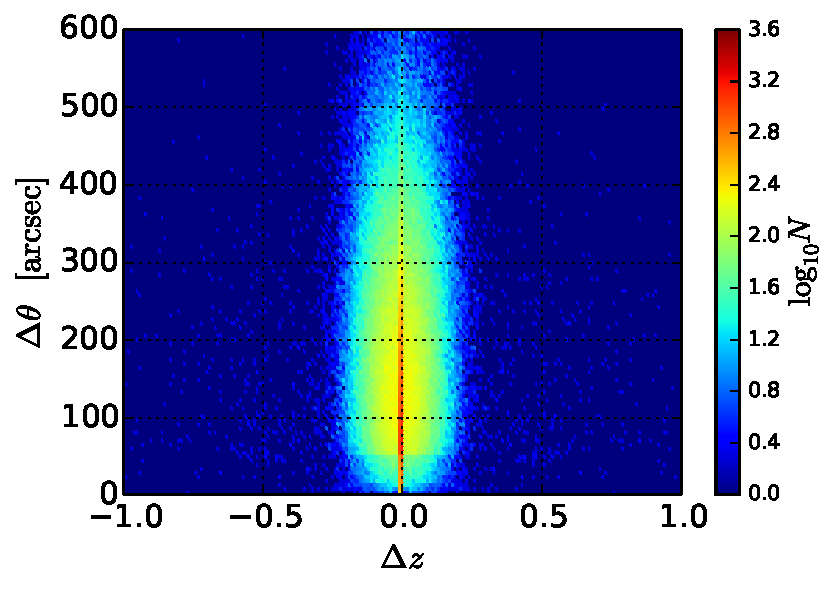
\includegraphics[width=0.6\linewidth]{figures/sdss/plane.pdf}
    \caption{\footnotesize{}Distribution of spectroscoped galaxies in the SDSS
    DR8 in angular size and redshift differences with the nearest neighbour
galaxy.\label{fig:plane}} \end{figure}
%
Nevertheless, the dense regions with more than one galaxy per $55''$ diameter
circle are partially incomplete in the SDSS spectroscopic sample.

We tried to implement this selection effect in our mock catalogue. For this, we
computed the local density in the field, taking all galaxies (spectroscoped or
not) in the neighbourhood of 1.5° around each galaxy, and at the same time, we
determine the fraction of galaxies that do not have a spectroscopic redshift,
to see the relation between spectroscopic completeness and photometric galaxy
number density. We expect to deduce a relation between the density field and
the fraction of fibre collisions. In the mock catalogue, we compute the same
density field and we apply the spectroscopic completeness relation estimated in
the SDSS sample to the mock. We have to remove galaxies that are close to
survey edges, because otherwise, there are missing galaxies and the
spectroscopic completeness will be affected. Edge galaxies are those lying
closer than 1.5 deg from the survey edges, which we measure in practice by
generating XXX random points within a circle of 1.5 deg radius around each
galaxy.

\remark{%
    We can generate samples of points at an angular distance $d$ to a point at
    position $(\alpha_0,\delta_0)$ using formulas of the spherical triangle.
    If we define a triangle by the pole, the point $(\alpha_0,\delta_0)$ and
    the point whose we want coordinates $(\alpha,\delta)$, we can write the
    following relations using the spherical triangle and its dual:
    %
    \begin{eqnarray}
        \sin\delta&=&\sin\delta_0\cos d + \cos\delta_0\sin d
        \cot\gamma\nonumber\\
        \sin\delta_0\cos\gamma&=&\cos\delta_0\cot{d}-\sin\gamma\cot\left(\alpha-\alpha_0\right)\nonumber\\
    \end{eqnarray}
    %
    where $\gamma$ is like a polar angle, which have all the values between 0
    and $2\pi$. We can rewrite:
    %
    \begin{eqnarray}
        \delta &=&
        \arcsin\left(\sin\delta_0\cos d + \cos\delta_0\sin d\cos\gamma\right)\nonumber\\
        \alpha-\alpha_0 &=& \arctan\left(\cfrac{\sin\gamma}{\cos\delta_0\cot{d}-\sin\delta_0\cos\gamma}\right)\nonumber\\
    \end{eqnarray}
    %
    There are problems at poles. For a $\gamma_0$ limit, angles can't be
    recovered with above formulas. Indeed, the problem appears when
    $\tan\Delta\alpha\rightarrow\infty$. So:
    %
    \begin{equation}
        \cos\delta_0\cot d -\cos\gamma_0\sin\delta_0 = 0
    \end{equation}
    %
    implying:
    %
    \begin{equation}
        \cos\gamma_0=\cfrac{1}{\tan d\tan\delta_0}
    \end{equation}
    %
    So to handle these limit cases, we summarize the correction for the
    differences in right ascensions by:
    %
    \begin{eqnarray}
        \Delta\alpha \rightarrow \Delta\alpha+\pi &\mathrm{if}&
        \mathrm{sign}\left(\delta_0\right)\cos\gamma \geqslant
        \mathrm{sign}\left(\delta_0\right)\cos\gamma_0\nonumber\\
    \end{eqnarray}

    Another way to draw circles on the sphere is to consider the point for
    which we want to know celestial coordinates around a given angular distance
    as the pole of a new coordinate system. In this system, points at a given
    distance of our central point are just points with $\pi/2-\delta$ and
    $\alpha$ running between 0 and $2\pi$. We now can determine cartesian
    coordinates of those points in this system and apply a rotation to go from
    the ``real'' system to the system where the central point is the pole. This
    can be easily done if we know the axis of rotation and the angle using
    quaternions, which is numerically more efficient than Euler angles.
}
%
We didn't see the trend we expected with the density field, so we thought that
it can be due to the large area in which we compute the fraction of
spectroscoped galaxies and we ran the same with a radius of 0.3°, but without
success too.

Moreover, including photometric redshifts in the mock catalogue and in MAGGIE
is very complex. For example, we measured the bias and dispersion of the
distribution of differences between spectroscoped and photometric redshifts in
the SDSS\@. \bartreffigure{redshift_difference} shows that while the dispersion
remains roughly constant, the bias increases with the spectroscoped redshift.
So some effects are not still under control when computing photometric
redshifts, and we should avoid their use in galaxy group algorithms when
possible. In the case of surveys where spectroscopic redshifts are not
available, the photometric redshifts should be as clean as possible.

\begin{figure}[hp]
    \begin{minipage}{\linewidth}
        \centering
        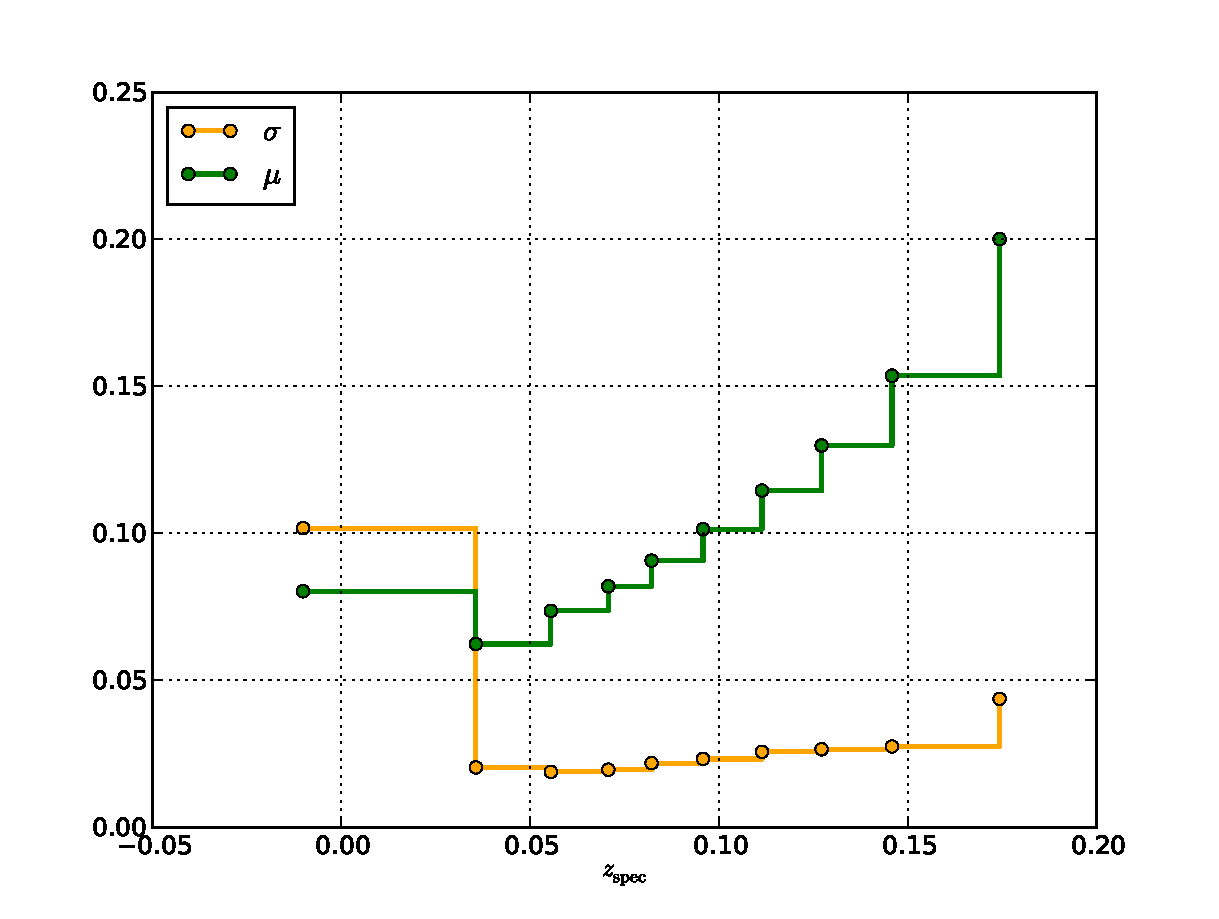
\includegraphics[height=0.4\textheight]{%
            figures/sdss/redshift_difference.pdf%
        }
        \captionof{figure}{Bias ($\mu$) and scatter ($\sigma$) of
        $z_\mathrm{phot} - z_\mathrm{spec}$.\label{fig:redshift_difference}}
    \end{minipage}
    \begin{minipage}{\linewidth}
        \centering
        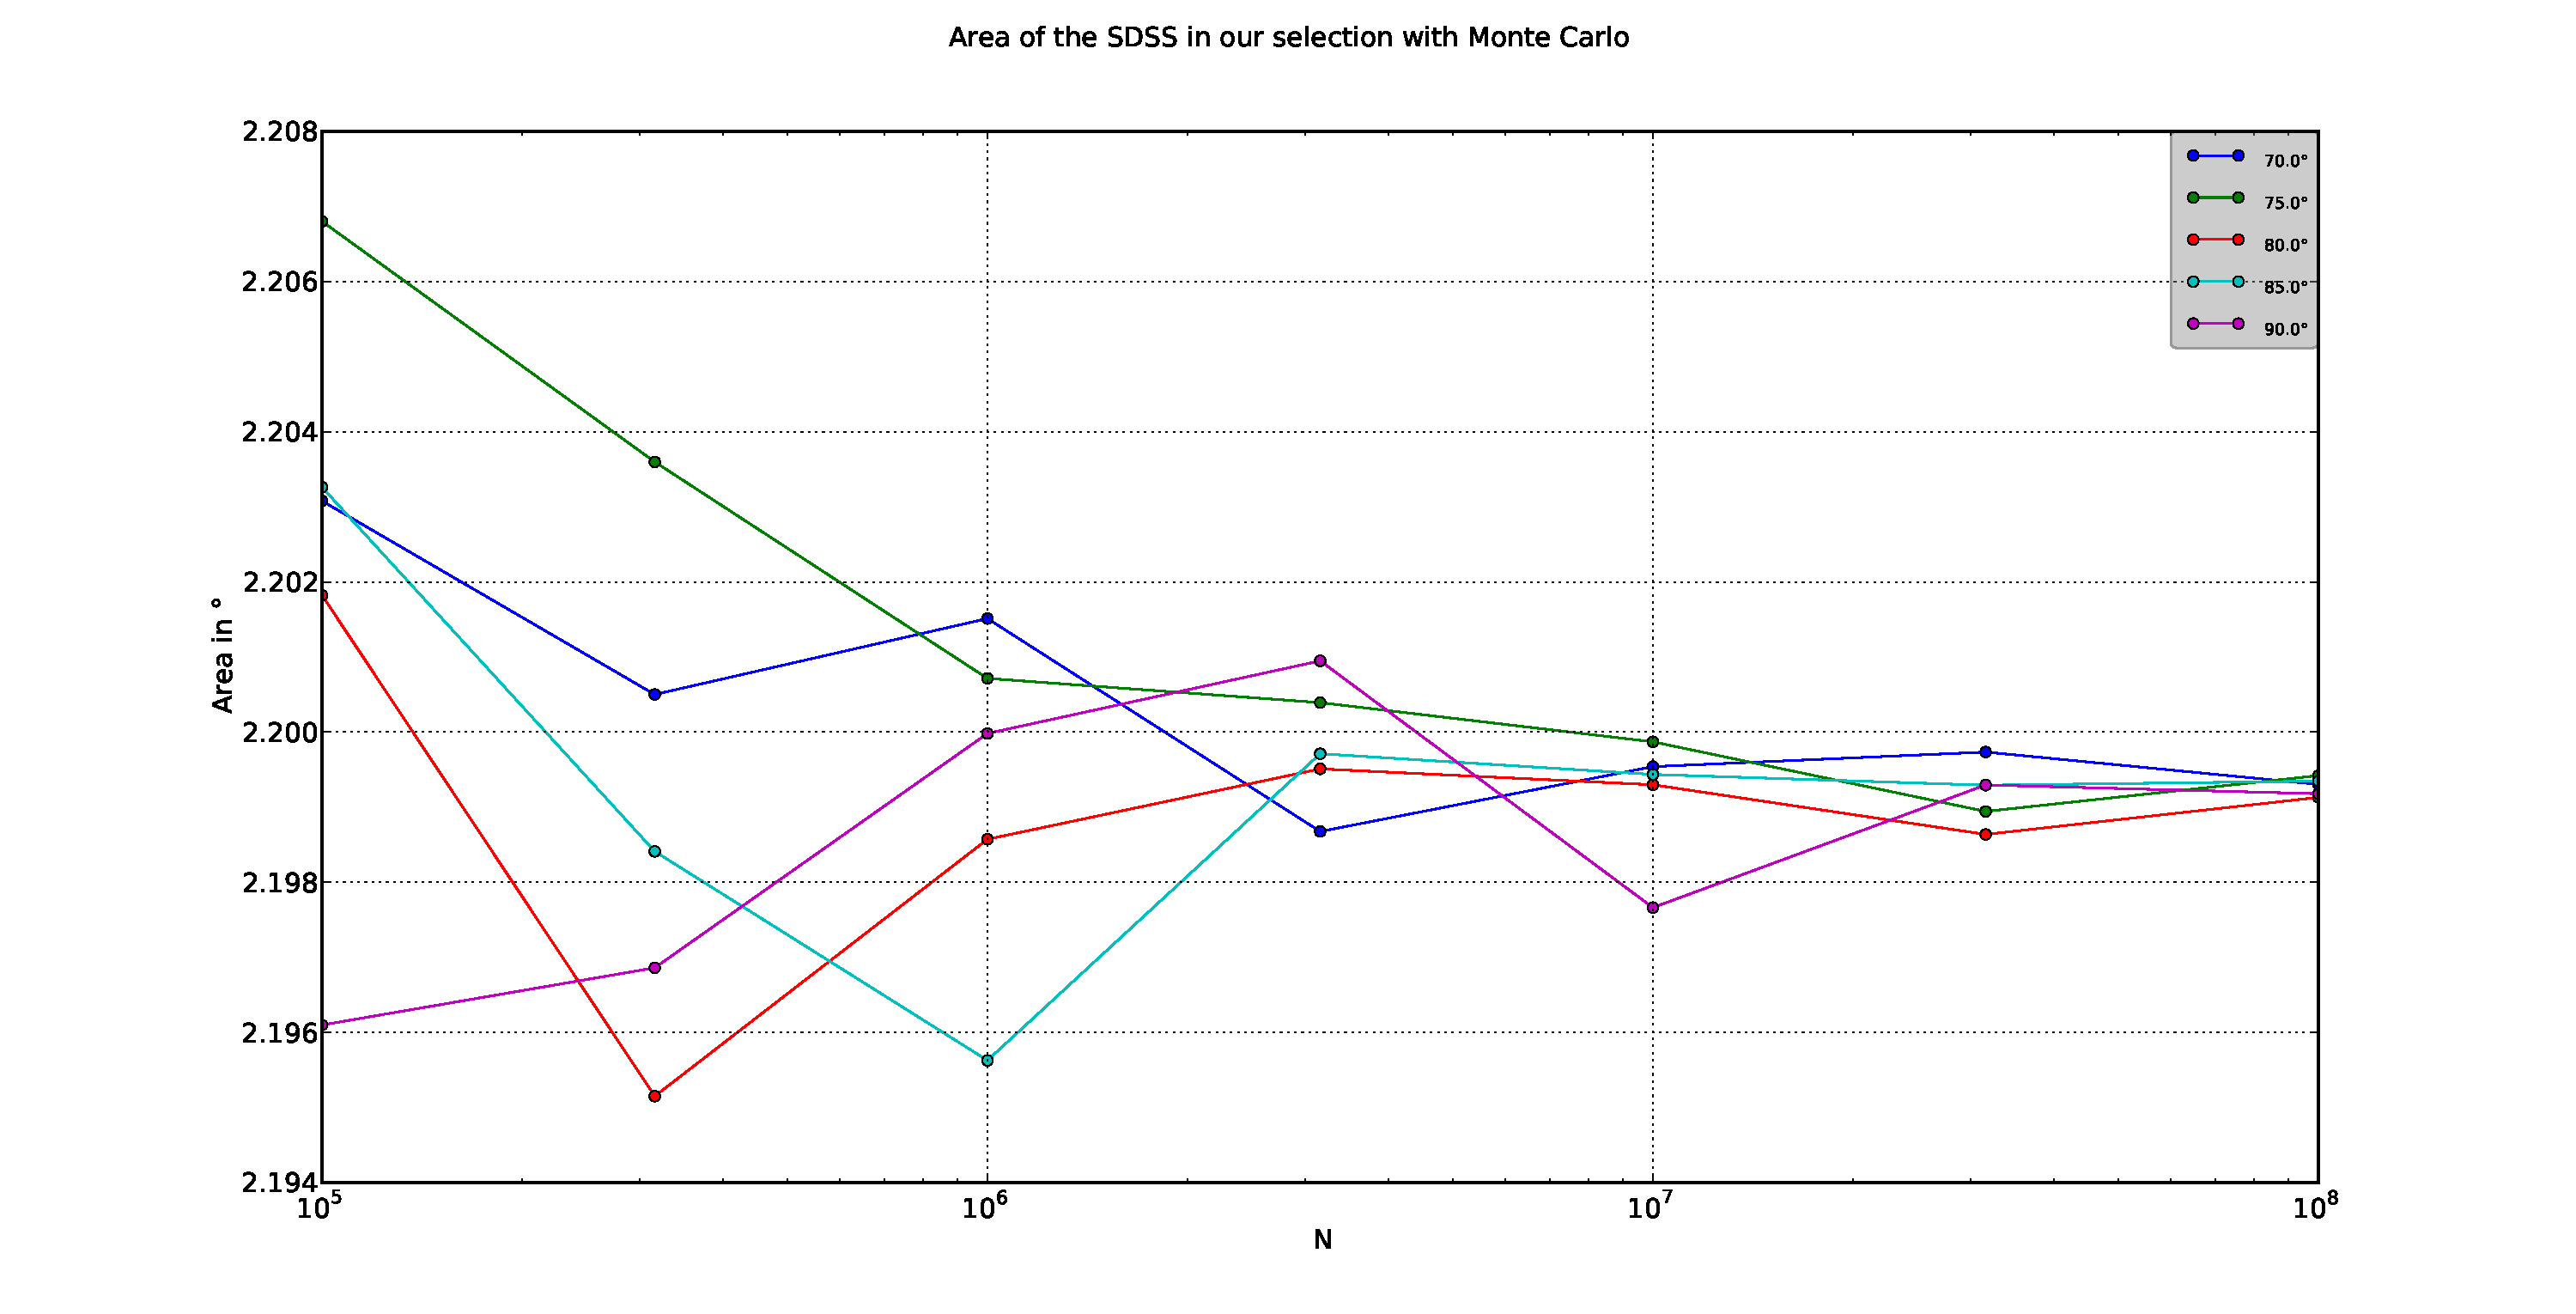
\includegraphics[height=0.4\textheight]{figures/sdss/SDSS_area}
        \captionof{figure}{Determination of the area of the SDSS for our
        selection with a Monte Carlo process. Results converge on a value of
    $2.1993\pm 0.0001$ steradians (i.e.\ roughly $7220\pm
\mathrm{\deg}^2$).\label{fig:sdss_area}}
    \end{minipage}
\end{figure}

\section{Coverage of the SDSS}

For many computations in this thesis, we need to determine the solid angle
covered by our galaxy sample. In the SDSS, the mask we constructed allows us to
do it easily by a Monte Carlo process.

First, we generate a number $N$ of points around a point of coordinates
$(\alpha_0, \delta_0)$ with a maximal angular separation $\theta_{\max}$ which
is larger than the maximal angular separation in our sample. The fraction of
points falling inside the mask gives us the fraction of the generated area
corresponding to the mask. This area is just
$\mathcal{S}=\int_0^{\theta_{\max}}\int_0^{2\pi}\sin\theta\dd{\theta}\dd{\phi}=
2\pi\left(1-\cos\theta_{\max}\right)$. We made this calculation for different
cone angles $\theta_{\max}$ and for different number of points to see if we
have a convergence in the value of the area. \bartreffigure{sdss_area} shows
that our geometry has a solid angle of $7220\pm1 \mathrm{\deg}^2$ but this
required five simulations with $10^8$ points.
%
\remark{%
    Generating points uniformly on the celestial sphere around a point of
    coordinates $(\alpha_0, \delta_0)$ to an angular distance $d$ can be done
    by assuming that this point is the upper pole of an other spherical system.
    In this situation, points follow $0\leqslant\theta\leqslant d$ and
    $0\leqslant\phi\leqslant2\pi$, assuming spherical coordinates and not
    celestial one. The azimuthal $\phi$ coordinates are generated as $2\pi U_1$
    where $U_1$ is a random variable following an uniform distribution between
    0 and 1. The latitude $\theta$ coordinates, follow
    $\left(p\left(\theta\right)=\cfrac{1}{2}\sin\theta\right)$ and are
    generated by $\theta=\arccos(2U_2-1)$, where $U_2$ is a variable following
    an uniform distribution with values between 0 and 1.

    Then, the points are rotated by quaternions to $(\alpha_0, \delta_0)$. The
    rotation axis is just the cross product between the pole vector and the
    vector defined by $(\alpha_0, \delta_0)$, and the rotation angle is
    $\cfrac{\pi}{2}-\delta_0$.
}

\section{Galaxy stellar masses}

In SDSS, contrary to coordinates, magnitudes or redshifts, stellar masses are
not measured by the SDSS pipelines. Instead, several teams have applied stellar
population models to the spectra and corrected their stellar masses from the
area subtended by the spectroscopic fiber to the entire galaxy, using the
apparent magnitudes within the fiber (fiberMag) and that extrapolated to the
entire galaxy (petroMag or modelMag). Indeed, contrary to coordinates,
magnitudes or redshifts, the stellar mass is not a direct observable. Its
estimation is based on the application of various stellar population models on
the galaxy spectrum observed by the SDSS\@. Several models exist, but they do
not provide the same estimation for a given galaxy. In
\bartreffigure{stellar_mass_models}, we compare eight models to have an order
of the inaccuracy of the stellar mass: FSPSGranWideDust, FSPSGranWideNoDust,
FSPSGranEarlyDust and FSPSGranEarlyNoDust from~\cite{Conroy+09}, PassivePort
and StarFormingPort from~\cite{Maraston+09}, PCAWiscM11 and PCAWiscBC03
from~\cite{Chen+12} and MPA-JHU from~\cite{Brinchmann+04, Kauffmann+03,
Tremonti+04}.

The principal discrepancies between the models come essentially from the
various stellar population synthesis (SPS) models involved in the fit of the
galaxy spectrum, necessary for the stellar mass estimation. But each model has
also some internal variations. For example,~\cite{Conroy+09} assume an early
star formation in galaxies for its FSPSGranEarlyNoDust (without dust extinction
correction) and FSPSGranEarlyDust (with dust extinction correction), while
FSPSGranWideDust and FSPSGranWideNoDust assume an extended star formation
history. As we can see, differences are relatively important: models using
different SPS have large dispersion in their estimation, while when using the
same SPS, stellar masses are coherent. Some models are also biased between each
other, but bias can be corrected and not considered in our analysis. Generally,
models agree to better than 0.3 dex, i.e.\ errors on individual masses are of
$0.3 / \sqrt{2} = 0.2$ dex. In particular, the MPA-JHU masses agree with all
others to typically better than 0.2 dex in $\sigma$.

\begin{figure}[htp]
    \centering
    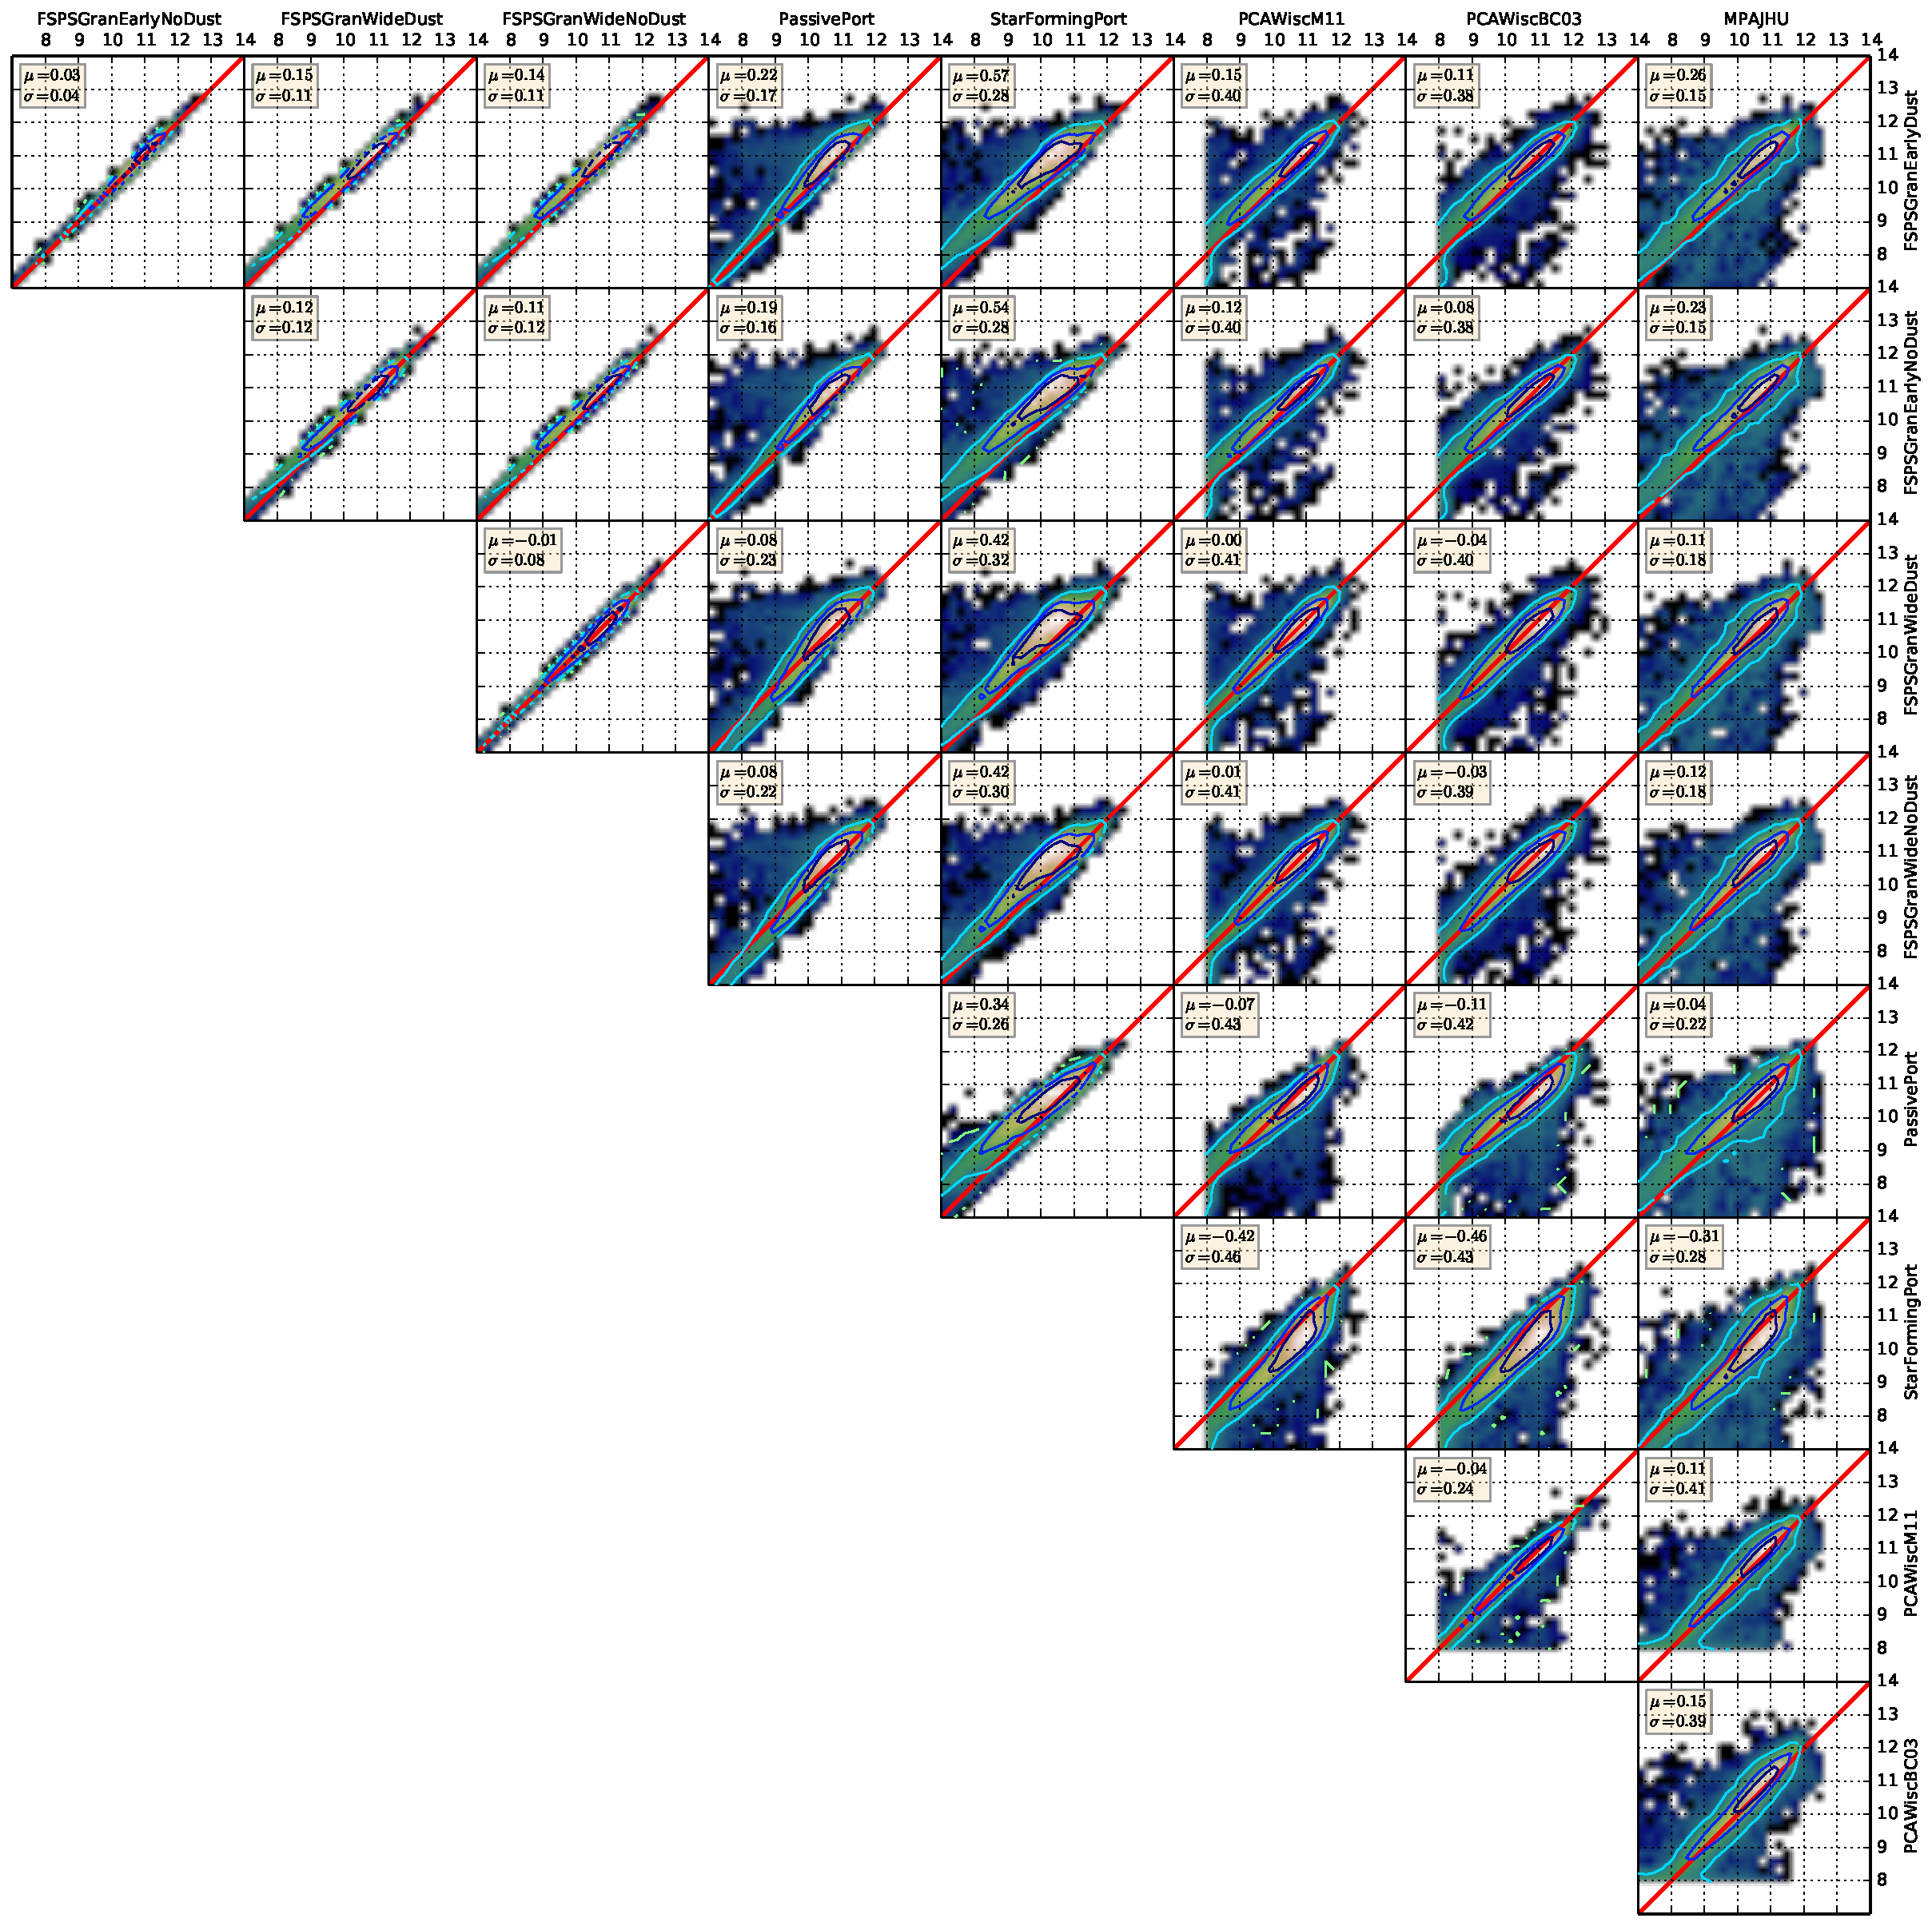
\includegraphics[width=\linewidth]{figures/sdss/stellar_mass_models.pdf}
    \caption{Comparison between stellar mass models applied onto galaxies from
        SDSS\@. Contours show the offsets in units of the scatter $\sigma$.
        Ordinates and abscissas are the logarithmic stellar masses of galaxies
        in the solar units. The upper left box shows the bias ($\mu$) and
        dispersion ($\sigma$) of the logarithmic difference between both
        models. The models are FSPSGranWideDust, FSPSGranWideNoDust,
        FSPSGranEarlyDust and FSPSGranEarlyNoDust \citep{Conroy+09},
        PassivePort and StarFormingPort \citep{Maraston+09}, PCAWiscM11 and
    PCAWiscBC03 \citep{Chen+12} and MPA-JHU~\citep{Brinchmann+04, Kauffmann+03,
Tremonti+04}.\label{fig:stellar_mass_models}}
\end{figure}

\section{Final galaxy sample}
\label{sec:final_galaxy_sample}

All previous sections are showing something important in the SDSS data:
observational errors can be important, and the automatic processing of this
data sometimes leads to false detections, artefacts\ldots, making analysis and
corrections complex.

Fortunately, recently in their FoF analysis of galaxy groups in the SDSS-DR10,
\cite{Tempel+14} had to deal too with such problems and the contamination they
introduce. Major problems are stars classified as galaxies, nearby large
galaxies fragmented into several galaxies or poor photometry of some galaxies
due to bright stars or bad sky level estimation in the neighbourhood. They
performed an impressive filtering on the sample by visually checking 30000
galaxies that were potentially problematic galaxies.~\cite{Tempel+14} thus
checked the following:
%
\begin{itemize}
    \item $10000$ apparently brightest galaxies (in $r$ band). For galaxies
        brighter than $m_r < 13.5$, about 10\% of the objects were spurious.
        For galaxies $13.5 < M_r < 14.5$, about 1\% were spurious entries; this
        fraction decreases with luminosity;
    \item $5000$ intrinsically brightest galaxies in the sample (< 1\% were
        spurious);
    \item $3000$ intrinsically faintest galaxies in the sample (to ensure the
        correctness of the faint-end of the luminosity function);
    \item all the sources with the spectroscopic class QSO\@;
    \item all the objects with \texttt{bestobjid} missing or not GALAXY\@. For
        these objects, they used \texttt{fluxobjid} if the matched photometric
        object was classified as a galaxy;
    \item all the objects for which the difference between $r$ band point
        spread function (PSF) magnitude and model magnitude was smaller than
        0.25 (thus further excluding some of the stellar sources in the
        catalogue);
    \item all the galaxies with the difference between $r$ band Petrosian and
        model magnitudes greater than 0.4;
    \item all the galaxy pairs that were closer than $5'$ (in order to remove
        double/multiple entries);
    \item the entries where the colour indices $g−r$, $r−i$, and $g−i$ had
        extreme values.
\end{itemize}

Finally,~\cite{Tempel+14} removed around $600$ galaxies, while $1400$ other
galaxies were flagged as having a bad photometry. We decided to use their
galaxy sample, since it covers exactly the same area we use and their
conscientious clean up of the SDSS-DR10 is difficult to surpass.

\subsection{Stellar masses}
\label{sub:stellar_masses}

Stellar masses are a major component of our algorithm, but~\cite{Tempel+14} did
not work with them, letting us the choice of the stellar masses to use. In
\bartreffigure{stellar_mass_models}, we show that there are large differences
between available models in the SDSS database. Estimations of some models are
different from the other and should not be used. A way to deal with this
problem is, for each galaxy in the sample, to use the median of the stellar
mass for all models. But sometimes, we don't have access to the stellar mass of
a galaxy and removing it from the sample will create supplementary
incompleteness. In such situations, we provide by default the
photometrically-based stellar mass estimation  of~\cite{Bell+03}. Those fitting
formulas allow to get the stellar mass of a galaxy directly from its color and
luminosity. Several colors are available to make the computation. We show in
\bartreffigure{bell_comparison} the stellar mass distribution for several
colors used on the formula of~\cite{Bell+03}. The $r-z$ color creates fewer
outliers in stellar masses than other bands. A possible explanation is that the
magnitude bands involved in the computation are less sensitive to dust
extinction and thus provide a more accurate estimation of stellar mass. So, we
adopt the stellar mass from $r-z$ color for those galaxies without spectral
mass estimates in the SDSS database.

\begin{figure}[htb]
    \centering
    \begin{minipage}{0.49\linewidth}
        \centering
        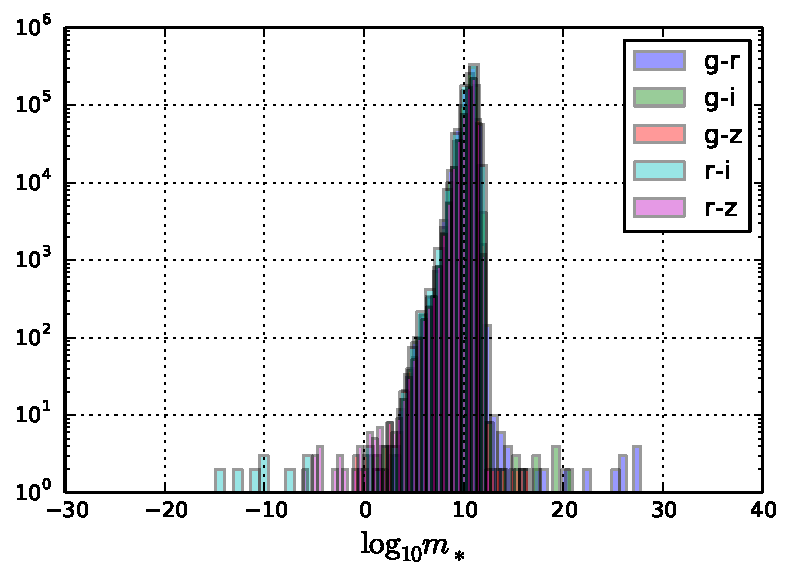
\includegraphics[width=\linewidth]{%
            figures/maggie_vs_sdss/bell_stellar_masses.pdf%
        }
        \captionof{figure}{The distribution of stellar masses for galaxies on
            the SDSS with the median of models described in
            \bartreffigure{stellar_mass_models} and the default value for
            galaxies without stellar mass estimations from~\cite{Bell+03} for
            different magnitude colors. The number of non-physical values for
            stellar masses is reduced by using the $r-z$ color, less affected
            by dust extinction and hence more
        accurate.\label{fig:bell_comparison}}
    \end{minipage}
    \begin{minipage}{0.49\linewidth}
        \centering
        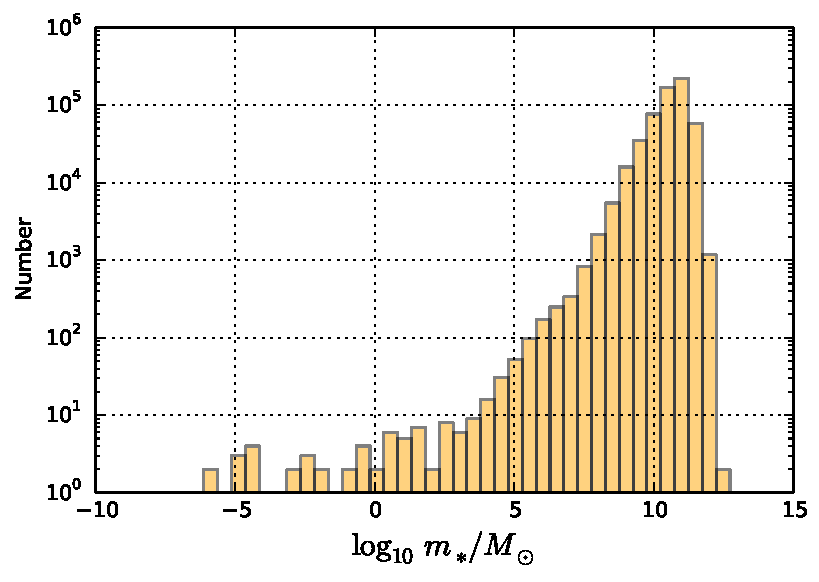
\includegraphics[width=\linewidth]{%
            figures/maggie_vs_sdss/sdss_stellar_masses_final.pdf%
        }
        \captionof{figure}{The distribution of stellar masses in solar units
            for our SDSS galaxy sample once chosen the $r-z$ color magnitude as
            default estimation. There are no high mass galaxies, but some
            stellar masses have unphysically low stellar masses. We keep them
            to avoid introducing supplementary incompleteness in the galaxy
        sample.\label{fig:stellar_mass_distribution}}
    \end{minipage}
\end{figure}

The resulting stellar mass distribution from our galaxy sample is shown in
\bartreffigure{stellar_mass_distribution}. No galaxies have too high stellar
masses, but a lot of them are very low and seems to not be physical. But we
can't remove them without introducing an incompleteness hence we keep them in
the sample.

\begin{figure}[htp]
    \centering
    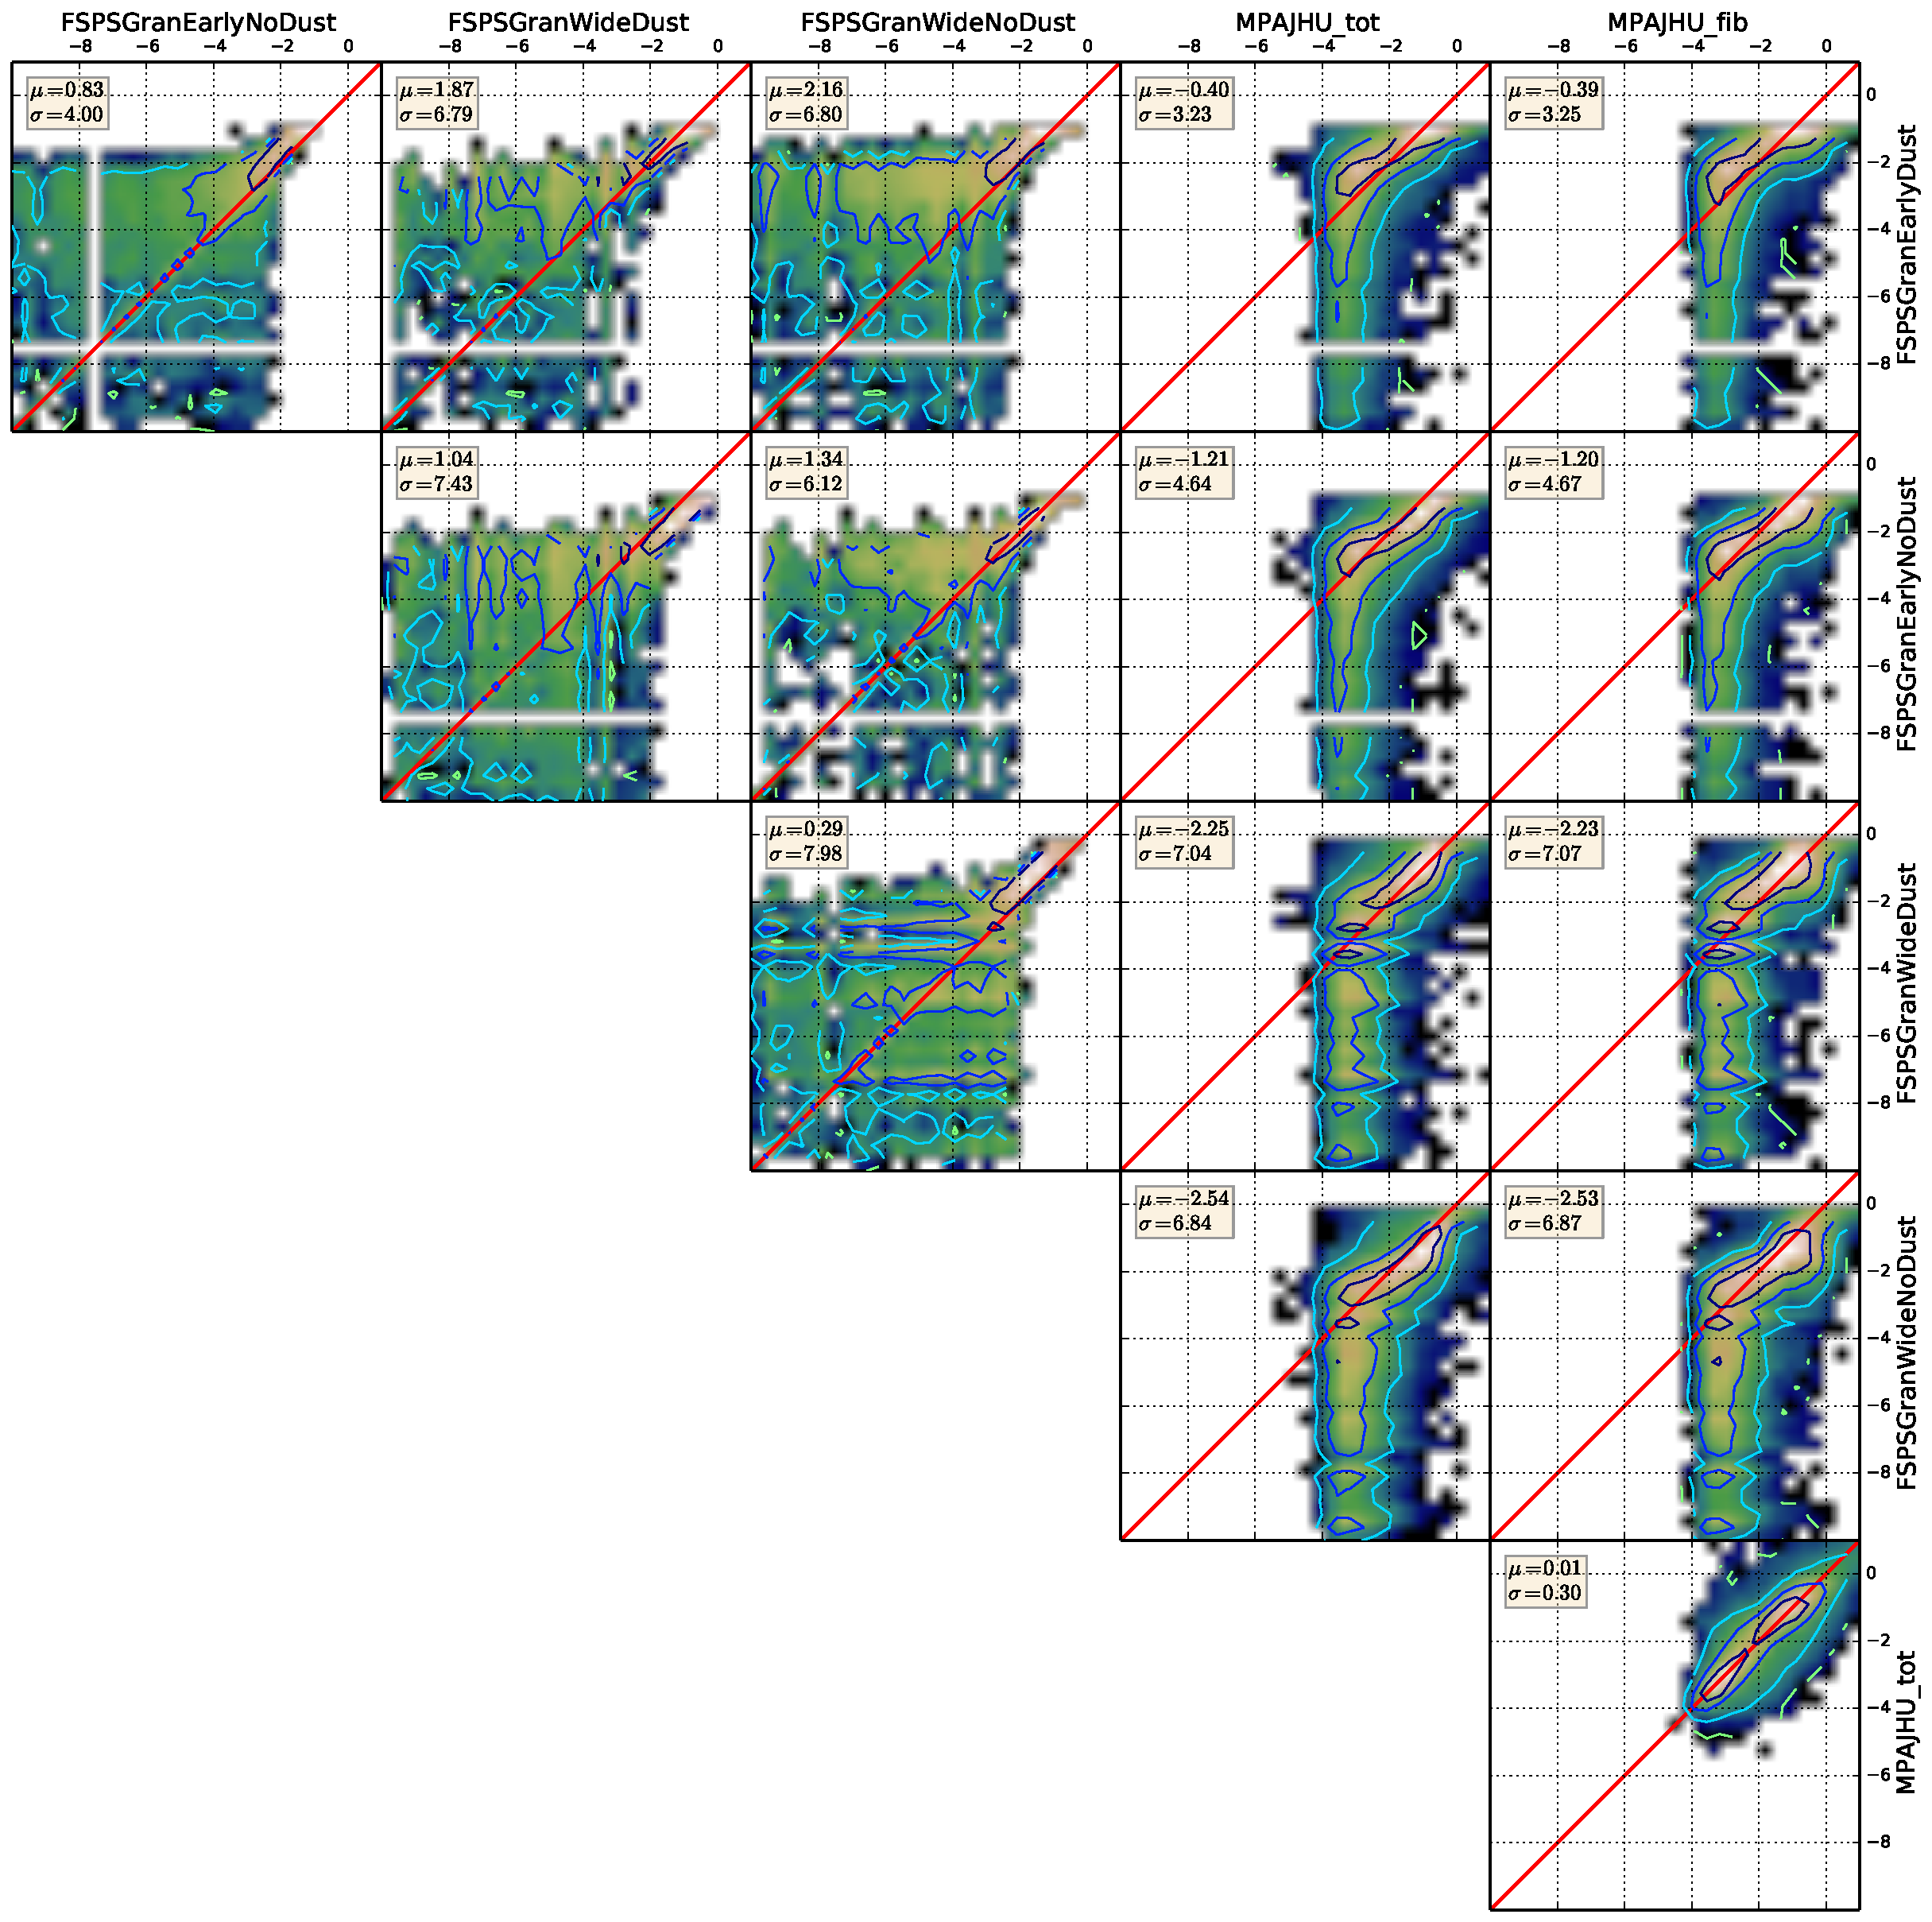
\includegraphics[width=\linewidth]{%
        figures/maggie_vs_sdss/ssfr_models.pdf%
    }
    \caption{Comparison of several specific star formation rate (SSFR) measures
        from different models. FSPSGranWideDust, FSPSGranWideNoDust,
        FSPSGranEarlyDust and FSPSGranEarlyNoDust from~\cite{Conroy+09} and
        MPA-JHU~\cite{Brinchmann+04, Kauffmann+03, Tremonti+04}. Two variants
        exist for MPA-JHU according to if the estimation is based on the region
        of the fiber (suffixed \emph{fib}) or is also extrapolated (suffixed
        \emph{tot}). Axes are $\log_{10} \mathrm{SSFR}$ in units of
        $\mathrm{Gyr}^{-1}$. We show also the bias and dispersion of the
        log-difference of models. FSPS models are not very consistent between
        one another and we do not use them. MPA-JHU are relatively coherent but
    we should prefer the \emph{total} estimation since with the fiber
estimation not all the stellar population of the galaxy is
probed.\label{fig:sfr_comparison}}
\end{figure}

\subsection{Star formation rate}
\label{sub:star_formation_rate}

Measures of the star formation rate suffer the same problems as stellar masses:
the different models (from the same teams) do not necessarily agree with one
another. The comparison of the SFR measures (shown as the specific star
formation rate, SSFR = SFR divided by stellar mass) is shown on
\bartreffigure{sfr_comparison}. Some models disappeared: PCAWiscM11 and
PCAWiscBC03 do not provide SFR estimates for galaxies, while PassivePort and
StarFormingPort produce null SFR values for too many galaxies. MPA-JHU has
several estimates of the SFR\@: one based only on informations acquired by
the fiber pointing to the galaxy to get its spectrum (suffixed by \emph{fib})
and the other where an extrapolation of the informations is done outside the
aperture (suffixed by \emph{tot}).

\bartreffigure{sfr_comparison} shows that the SSFR values from the different
FSPS models are not consistent with one another, hence we did not use them in
our analysis. The bias and scatter between both models of MPA-JHU are small,
making them good measure of the SSFR of galaxies. Our preference goes to the
\emph{total} model, since the extrapolation used by the authors (at roughly
constant SSFR) must be better than none.

\begin{figure}[htb]
    \centering
    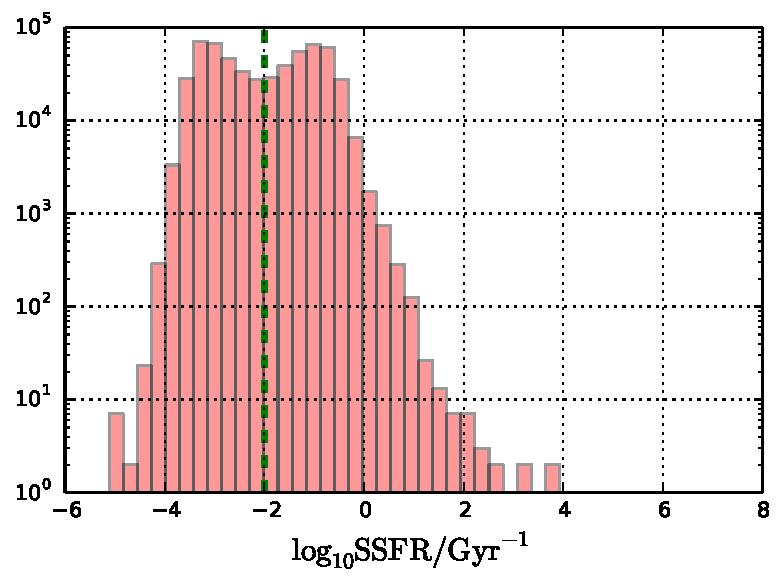
\includegraphics[width=0.8\linewidth]{%
        figures/maggie_vs_sdss/sfr_distribution.pdf%
    }
    \caption{The distribution of SSFR from the MPA-JHU model. We can see a
    bi-modality in the distribution, splitting galaxies into star forming
and passive galaxies (the \emph{green dashed} line shows the
separation).\label{fig:ssfr_distribution}}
\end{figure}

The resulting distribution of the SSFR in \bartreffigure{ssfr_distribution}
shows that galaxies can be classified into two categories: a star forming
population where an important fraction of the galaxy stellar mass is produced
in a time scale of $1$ Gyr and a passive one, where ongoing or recent star
formation represents a small fraction of its stellar mass. The green line in
\bartreffigure{ssfr_distribution} shows this limit. It will be useful when
searching if there is a modulation with the environment of the fraction of
young galaxies.

% vim: set tw=79 :
